\subsection*{Figures}

\begin{figure}[htb!]
\centering
	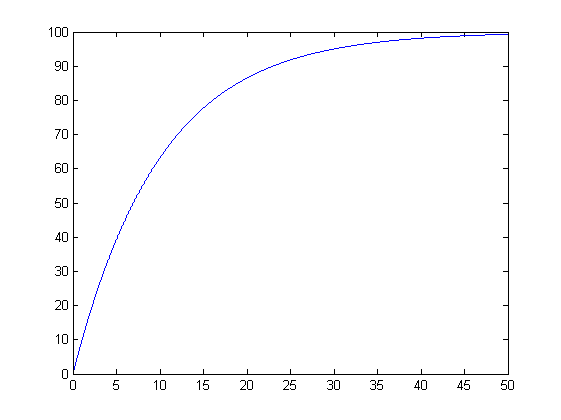
\includegraphics[width=0.5\textwidth]{mshape.png}
\caption{The shape of the Goel-Okumoto model}
\label{goelokumoto}
\end{figure}

\begin{figure}[htb!]
\centering
	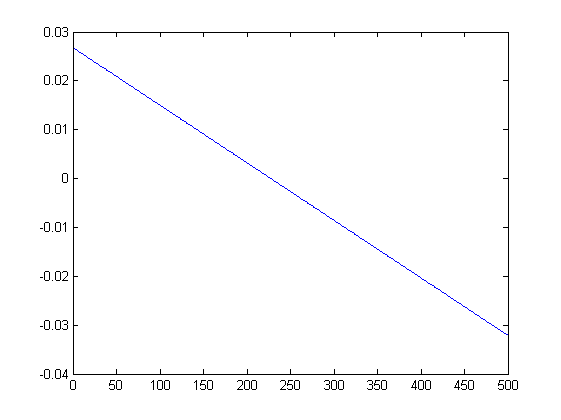
\includegraphics[width=0.5\textwidth]{jmshape.png}
\caption{The shape of the Jelinski-Moranda model}
\label{jelinskimoranda}
\end{figure}

\begin{figure}[htb!]
\begin{center}
	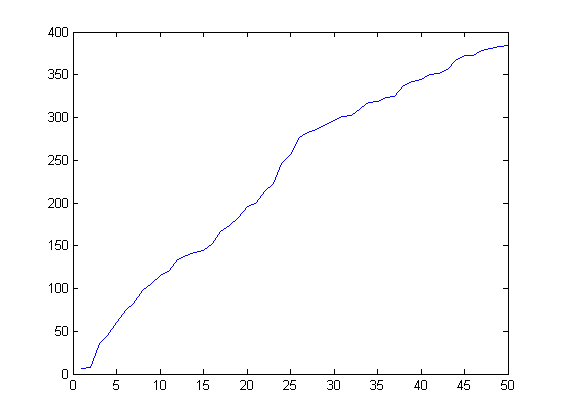
\includegraphics[width=0.5\textwidth]{cumsumgodata1plot.png}
\caption{The cumulative sum of failures found in TROPICO R-1500 in 50 weeks.}
\end{center}
\label{cumulativegodata1}
\end{figure}

\begin{figure}[htb!]
\begin{center}
	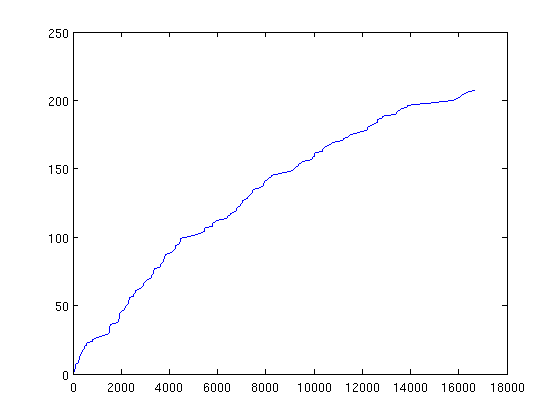
\includegraphics[width=0.5\textwidth]{cumsumjmdata2.png}
\caption{The cumulative sum of the time between failures as well as the failures found in an analyzed system, long time.}
\end{center}
\label{cumulativejmdata2}
\end{figure}


\begin{figure}[htb!]
\begin{center}
	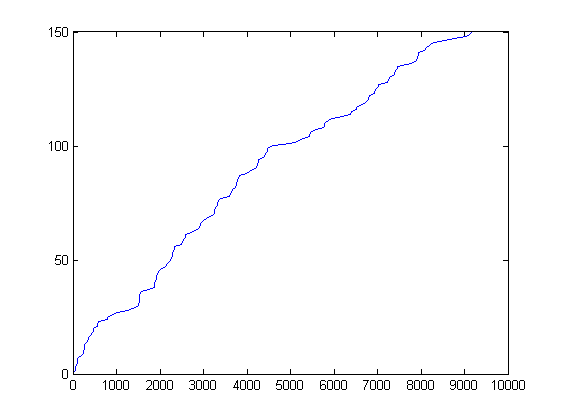
\includegraphics[width=0.5\textwidth]{cumsumjmdata1plot.png}
\caption{The cumulative sum of the time between failures as well as the failures found in an analyzed system, short time.}
\end{center}
\label{cumulativejmdata1}
\end{figure}

\clearpage
\subsection*{Tables}

\begin{table}[!htb]
	\centering
	\caption{$N_{future}$ and $N_{tot}$ with subjective and GO-estimation as well as real values.}
	\label{goelokumototable}	
    \begin{tabular}{|l|l|l|}
        \hline
        ~ & $N_{future}$ & $N_{tot}$ \\ \hline
        Subjective Estimation            & 500   & 600 		\\ 
        GO estimation                    & 458.1 & 547.5	\\ 
        Actual values                    & 459 	 & 461		\\ 
        \hline
    \end{tabular}
\end{table}

\begin{table}[!htb]
	\centering
	\caption{$N_{future}$ and $N_{tot}$ with subjective and JM-estimation as well as real values.}
	\label{jelinskimorandatable}	
    \begin{tabular}{|l|l|l|}
        \hline
        ~ & $N_{future}$ & $N_{tot}$ \\ \hline
        Subjective Estimation            & 230   & 500 		\\ 
        JM estimation                    & N/A   & 226.5	\\ 
        Actual values                    & 200 	 & 207		\\ 
        \hline
    \end{tabular}
\end{table}